\chapter{Estadística}
\section{Estadística descriptiva}
\subsection{Conceptos}
\begin{itemize}[itemsep=0pt,parsep=0pt,topsep=0pt,partopsep=0pt]
    \item \textbf{Estadística}: rama de las Matemáticas encargada de los métodos y procedimientos de recogida, clasificación, síntesis y análisis de datos y su posterior interpretación. Se pueden distinguir, entre sus ramas principales:
    \begin{itemize}[itemsep=0pt,parsep=0pt,topsep=0pt,partopsep=0pt]
        \item\textbf{Descriptiva}: describe, analiza y representa datos según medidas matemáticas y gráficos, que muestran la información obtenida.
        \item\textbf{Inferencial}: permite, a través de datos descriptivos, efectuar estimaciones, predicciones o generalizaciones de una población.
    \end{itemize}
    \item \textbf{Individuo/Elemento}: ente con una información a estudiar.
    \item\textbf{Población}: conjunto de individuos con propiedades comunes. Pueden ser:
    \begin{itemize}[itemsep=0pt,parsep=0pt,topsep=0pt,partopsep=0pt]
        \item \textbf{Finita}: tiene un tamaño limitado.
        \item\textbf{Infinita}: tiene un tamaño que tiende al infinito.
    \end{itemize}
    \item\textbf{Muestra}: subconjunto representativo de una población.
    \item\textbf{Parámetro}: función definida sobre los valores numéricos de características medibles de una población.
    \item\textbf{Estadístico}: función definida sobre los valores numéricos de una muestra.
\end{itemize}
\subsubsection{Variable}
\paragraph{Variable o carácter} Propiedad, rasgo o cualidad de los elementos de una población. Tienen los siguientes elementos:
\begin{itemize}[itemsep=0pt,parsep=0pt,topsep=0pt,partopsep=0pt]
    \item \textbf{Modalidad}: valor de una variable, diferentes situaciones de un carácter.
    \item\textbf{Clase o intervalo}: conjunto de una o más modalidades en los que se verifica que cada modalidad pertenece a un intervalo.
    \item\textbf{Marcas de clase}: valor central (media) de un intervalo.
\end{itemize}
\subparagraph{Tipos de variable}
\begin{itemize}[itemsep=0pt,parsep=0pt,topsep=0pt,partopsep=0pt]
    \item \textbf{Cualitativa nominal}: sirve en categorización y etiquetado de elementos. La modalidad no tiene valor numérico. Sólo permite hallar la moda.
    \item\textbf{Cualitativa ordenada/Cuasicuantitativa}: sirve en categorización y etiquetado de elementos. La modalidad es un número que codifica a una cualidad. Pueden ordenarse.
    \item\textbf{Cuantitativa}: da una magnitud de una medición. Tiene un valor numérico que es la cantidad de una magnitud:
    \begin{itemize}[itemsep=0pt,parsep=0pt,topsep=0pt,partopsep=0pt]
        \item \textbf{Discretos}: son enteros ($\Z$). Pueden hacerse operaciones de suma, resta, producto, orden y conteo.
        \item\textbf{Continuos}: son números reales ($\R$). Pueden hacerse operaciones de suma, resta, división, orden, integración, derivación y limite.
    \end{itemize}
\end{itemize}
\subsubsection{Tablas estadísticas}
Elementos de ordenación de datos que se componen de:
\begin{itemize}[itemsep=0pt,parsep=0pt,topsep=0pt,partopsep=0pt]
    \item \textbf{Frecuencia absoluta} ($n_i$): número de repeticiones de un valor o modalidad.
    \item\textbf{Frecuencia absoluta acumulada} ($N_i$): unicamente calculable en variables que se puedan sumar. Número de elementos cuya modalidad es igual o menor al valor $x_i$.
        \[ N_i = \sum_{j=1}^{i}n_j \]
    \item\textbf{Frecuencia relativa} ($f_i$): cociente resultante de dividir la frecuencia absoluta de la modalidad y el total de observaciones
        \[ f_i = \dfrac{n_i}{n} \]
    \item\textbf{Frecuencia relativa acumulada} ($F_i$): sólo se puede calcular en variables que permitan sumar. Suma de las frecuencias relativas de las modalidades iguales o inferiores a $x_i$.
        \[ F_i = \sum_{1}^{i}f_i \]
    \item\textbf{Distribución de frecuencias}: conjunto de clases ordenadas junto a sus frecuencias.
\end{itemize}
\subsubsection{Diagramas}
\begin{itemize}[itemsep=0pt,parsep=0pt,topsep=0pt,partopsep=0pt]
    \item \textbf{Pictogramas}: expresan información mediante dibujos alusivos al tema a estudio. Los dibujos están escalados, siendo el área proporcional a la frecuencia.
    \item\textbf{Sectores}: división de un círculo en las clases existentes, con arcos proporcionales a las frecuencias. Si se comparan dos poblaciones, el radio de las semicircunferencias es proporcional al tamaño de las poblaciones.
        \[ r_2 = r_1\cdot\sqrt{\dfrac{n_2}{n_1}} \]
    \item\textbf{Barras}: ordenan a la modalidad en un eje y da la frecuencia en el otro.
    \item\textbf{Histograma}: diagrama de barras utilizado en representación de intervalos.
    \begin{itemize}[itemsep=0pt,parsep=0pt,topsep=0pt,partopsep=0pt]
        \item \textbf{Base}: anchura correspondiente al intervalo.
        \item\textbf{Altura}: proporciona a la frecuencia.
            \[h = \dfrac{f_i}{base}\]
    \end{itemize}
    \item\textbf{Polígono de frecuencias}: obtenido del histograma, área delimitada por una recta que pasa por el punto medio de todas las barras.
    \item\textbf{Diagramas acumulados}: representan frecuencias acumuladas. Existen de dos tipos:
    \begin{itemize}[itemsep=0pt,parsep=0pt,topsep=0pt,partopsep=0pt]
        \item \textbf{Variables discretas}: diagrama de barras escalonado siempre creciente.
        \item\textbf{Variables continuas}: polígono de frecuencias siempre creciente.
    \end{itemize}
\end{itemize}
\begin{table}[H]
    \begin{tabular}{cccc}
        \rowcolor{black}\textcolor{White}{\textbf{Variable}}&\textcolor{White}{\textbf{Cuantitativa}}&&\textcolor{White}{\textbf{Cualitativa}}\\
        \rowcolor{black}&\textcolor{White}{\textbf{Continua}}&\textcolor{White}{\textbf{Discreta}}&\\
        Diagrama&Diferencial: histograma&Diferencial: Barras&Pictogramas\\
        &Polígono de frecuencias&Integral: Diagrama acumulado&Sectores\\
        &Integral: diagramas acumulados&&Barras\\
        \hline
    \end{tabular}
\end{table}
\subsubsection{Valores centrales}
Los valores centrales traten de hacer ver que es lo característica de una muestra. De esta forma, son valores representativos de la muestra, tratan de resumir información en unos pocos datos generalizando la información.
\paragraph{Media}: Valor obtenido como la suma de todos los datos entre el número de observaciones. Queda a la misma distancia de todos los datos:
\begin{center}
    \begin{equation}
        \bar{X} = \dfrac{\sum_{1}^{n}x_j}{n}
    \end{equation}
    \captionof{Ecuacion}{Cálculo de la media.}
\end{center}
\subparagraph{Modos de cálculo}
\begin{itemize}[itemsep=0pt,parsep=0pt,topsep=0pt,partopsep=0pt]
    \item \textbf{Datos no tabulados}: se suman todos y se divide entre el número de datos.
    \item\textbf{Datos en tablas}: se suma el producto de cada datos por su frecuencia absoluta y se divide entre la suma de todas las frecuencias.
    \item\textbf{Datos en intervalos}: se hace lo mismo que en el caso anterior, pero utilizando las marcas de clase.
\end{itemize}
\paragraph{Mediana}: Valor obtenido como el valor central de la serie ordenada de todos los datos. Los modos de cálculo, en todos los casos se utilizan frecuencias absolutas o relativas acumuladas. La modalidad que está más cercana al 50 \% y supere este valor es la mediana. Si no estan tabulados, basta con ordenarlos y buscar la mitad. Si la cantidad de valores es par, se hará semisuma de los valores centrales, mientras que si es impar, se coge el valor central.
\paragraph{Moda}: Valor que se calcula como la modalidad que más se repite, la que tiene la frecuencia absoluta máxima.
\subsubsection{Valores de dispersión}
Los valores de dispersión indican si los datos de una variable están o no muy agrupados, o dispersos con respecto a los valores centrales, permitiendo juzgar si la información que moda, media y mediana ofrecen es correcta o no.
\paragraph{Rango}: Valor que indica la amplitud del intervalo para los que se considera la variable. Se obtiene como la diferencias entre el valor más alto y el más bajo de la variable. Se ve afectada por observaciones extremas, no disminuyendo si aumenta el número de observaciones.
\begin{center}
    \begin{equation}
        \mbox{Rango} = x_n - x_1
    \end{equation}
    \captionof{Ecuacion}{Cálculo del rango.}
\end{center}
\paragraph{Varianza}: Media de las diferencias cuadráticas de los valores con respecto a su media aritmética. Debido a que da valores que son las del cuadrado de la variable, se usa más la desviación típica. No es recomendable usarla si la media no es buena como medida de tendencia central. Son muy sensibles ante la modificación de un solo dato.
\begin{center}
    \begin{equation}
        S^2 = \dfrac{\sum_{i = 1}^{n}\left(x_1-\bar{X}\right)}{n}
    \end{equation}
    \captionof{Ecuacion}{Cálculo de la varianza.}
\end{center}
\paragraph{Desviación típica}: raíz cuadrada de la varianza. No es recomendable usarla si la media no es buena como medida de tendencia central. Son muy sensible ante la modificación de un solo dato.
\begin{center}
    \begin{equation}
        S = \sqrt{\mbox{Var}}
    \end{equation}
    \captionof{Ecuacion}{Cálculo de la desviación típica.}
\end{center}
\paragraph{Coeficiente de variación o de Pearson}: Valor obtenido de dividir la desviación típica entre la media. Elimina la dimensionalidad, permitiendo comparar variables diferentes. Sólo se puede aplicar a números positivos. Aunque no le afectan las modificaciones de escala, si se le suma a una medida una cantidad positiva, el nuevo Coeficiente de variación es menor que el anterior.
\begin{center}
    \begin{equation}
        CV = \dfrac{S}{\bar{X}}
    \end{equation}
    \captionof{Ecuacion}{Cálculo del coeficiente de variación.}
\end{center}
\subsubsection{Estadísticos de posición}
Valores de una variable que alcanzan un porcentaje o posición determinadas.
\paragraph{Percentiles}: Valor de una variable que deja por debajo de si un porcentaje determinado de la población. Se puede calcular:
\begin{itemize}[itemsep=0pt,parsep=0pt,topsep=0pt,partopsep=0pt]
    \item \textbf{Datos no tabulados}: a partir del total, se halla el valor que es el porcentaje y se busca.
    \item\textbf{Datos tabulados}: siguen el proceso anterior.
    \item\textbf{Datos en intervalos}: con los procesos anteriores se halla el intervalo y luego se interpola
\end{itemize}
\begin{center}
    \begin{equation}
        P_k = x_{i-1} + \dfrac{n\dfrac{\%}{100} - N_{i-1}}{n_i}\cdot\mbox{Rango}\qquad P_k = x_i + \dfrac{\mbox{Rango}}{n_i}\cdot\left(\mbox{Total}\cdot\% - N_{i-1}\right)
    \end{equation}
    \captionof{Ecuacion}{Cálculo de los percentiles.}
\end{center}
\paragraph{Cuartiles}: Se consideran como percentiles especiales:
\begin{itemize}[itemsep=0pt,parsep=0pt,topsep=0pt,partopsep=0pt]
    \item \textbf{Cuartil primero} ($Q_1$): es el percentil 25, deja por debajo a un cuarto de la población.
    \item \textbf{Cuartil segundo} ($Q_2$): es el percentil 50, deja por debajo a la mitad de la población, siendo la mediana.
    \item \textbf{Cuartil tercero} ($Q_3$): es el percentil 75, deja por debajo a tres cuartas partes de la población.
\end{itemize}
\paragraph{Rango intercuartílico} (IQR): diferencia entre el tercer y primer cuartil. Determina si hay datos atípicos (\textit{outlier}), de manera que todo dato atípico es aquel cuay diferencia con el cuartil primero o tercero es 1.5 veces el IQR.
\section{Probabilidad}
La \textbf{probabilidad} es la rama de las Matemáticas que estudia la relación entre el número de veces que ocurre un suceso y el número de veces en que podría suceder, siempre y cuando éste se dé por azar.
\subsection{Suceso, Espacio muestral}
\begin{itemize}[itemsep=0pt,parsep=0pt,topsep=0pt,partopsep=0pt]
    \item \textbf{Espacio muestral} ($\Omega$, E): conjunto de todos los resultados posibles que pueden suceder en un determinado proceso.
    \item\textbf{Suceso} ($A, B, C \dots$): cada uno de los subconjuntos del espacio muestral. Los tipos de sucesos son:
    \begin{itemize}[itemsep=0pt,parsep=0pt,topsep=0pt,partopsep=0pt]
        \item \textbf{Elemental}:  suceso que no puede ser desgajado en otro suceso más simple. La recopilación de todos estos da el espacio muestral.
        \item\textbf{Suceso unión} ($P_{\left( A\cup B\right) }$): conjunto de sucesos elementales que bien pueden ocurrir en A o pueden ocurrir en B.
            \[ P_{\left( A\cup B\right) } = P_A + P_B  -P_{\left( A\cap B\right) }\]
        \item\textbf{Suceso intersección} ($P_{\left( A \cap B\right) }$): conjunto de sucesos elementales que cumple que se den en el suceso A y B.
             \[ P_{\left( A\cap B\right) } = P_A - P_B + P_{\left( A\cup B\right) } \]
         \item\textbf{Suceso diferencia} ($P_{\left( A\setminus B\right) }$): conjunto de sucesos elementales que cumplen que se dan en A pero no en B.
            \[ P_{\left( A\setminus B\right) } = P_A - P_B = P_{\left( A\cap \bar{B}\right) } \]
        \item\textbf{Suceso diferencia simétrica} ($P_{\left( A\bigtriangleup B\right) }$): conjunto de sucesos elementales que cumple que están en A no están en B, y los que están en B no están en A.
            \[ P_{\left( A\bigtriangleup B\right) } = P_{\left( A\cup B\right) }\setminus P_{\left( B\cap A\right) } \]
        \item\textbf{Suceso contrario} ($P_{\bar{A}}$): conjunto de sucesos elementales que cumplen que no se da A.
            \[ P_{\bar{A}} = 1- P_A \]
    \end{itemize}
\end{itemize}
\subsection{Regla de Laplace}
La \textbf{regla de Laplace} afirma que la probabilidad de que un suceso A resulte es el cociente entre los sucesos favorables a A y el total de sucesos elementales que conforman el espacio muestral.
\begin{center}
    \begin{equation}
        P_A = \dfrac{\mbox{Sucesos favorables A}}{\Omega}
    \end{equation}
    \captionof{Ecuacion}[Regla de Laplace]{Regla de Laplace. $\omega$ indica el total del espacio muestral.}
\end{center}
No obstante, existen varias excepciones a la Regla de Laplace:
\begin{itemize}[itemsep=0pt,parsep=0pt,topsep=0pt,partopsep=0pt]
    \item Para poder aplicar la regla de Laplace, es necesario que todos los sucesos tengan un espacio muestral donde sus subconjuntos sean elementales y equiprobables (tienen la misma probabilidad de resultar). De esta manera, no es aplicable a, por ejemplo, dados trucados.
    \item No se puede aplicar a aquellos sucesos de sea infinito y/o el número de sucesos favorables sea infinito (daría lugar a una indeterminación no resoluble).
\end{itemize}
\subsection{Leyes de Kolmogorov}
Las leyes de Kolmogorov son tres axiomas que definen cuando se puede hablar íntegramente de probabilidad:
\begin{itemize}[itemsep=0pt,parsep=0pt,topsep=0pt,partopsep=0pt]
    \item \textbf{Primer axioma}: La probabilidad de cualquier suceso está definida entre los valores positivos del intervalo de 0 a 1, ambos incluidos.
        \[ P_{\left( A\right) }  \subset \left[ 0,1 \right] \subset \R \]
    \item\textbf{Segundo axioma}: la probabilidad del suceso seguro, que siempre se da, es 1. La probabilidad del suceso improbable, su contrario, es 0.
        \[ P_{\left( E \right) } = 1 \qquad P_{\left( \bar{E} \right) } = 0 \]
    \item\textbf{Tercer axioma}: la probabilidad del suceso unión es la suma de las probabilidad A y B menos la probabilidad del suceso intersección. La probabilidad de sucesos disconjuntos es la suma de sus probabilidades.
        \[ P\left[ \bigcup_{i = 1}^{\infty} A_i\right] = \sum_{i = 1}^{\infty} P_{\left( A_i\right) }  \]
\end{itemize}
\subsection{Función de probabilidad}
La función de probabilidad ($fn(e)$) se define como:
\begin{center}
    \begin{equation}
       fn(e) = \dfrac{\mbox{Ocurrencias de e}}{n}
    \end{equation}
    \captionof{Ecuacion}[Función de probabilidad]{Función de probabilidad. Debido a los problemas que pueden desarrollarse, se suele usar la regla de Laplace, muy similar.}
\end{center}

Se puede definir una serie de propiedades de la probabilidad:
\begin{itemize}[itemsep=0pt,parsep=0pt,topsep=0pt,partopsep=0pt]
    \item Sea cual sea el suceso aleatorio A, su probabilidad está entre 0 y 1.
        \[ 0 \leq P_A \leq 1 \]
    \item La probabilidad del espacio muestral es 1.
    \item La probabilidad del espacio muestral vacio ($\Omega = \left\lbrace \right\rbrace $)  es cero.
    \item Si A y B son dos sucesos disjuntos  (y siendo el suceso intersección nulo $P_{\left( A\cap B\right) } = 0$ ), esto es, que no pueden ocurrir a la vez, el suceso unión es la suma de probabilidades
        \[ P_{\left( A\cap B\right) } = 0 \iff P_{\left( A\cup B\right) } = P_A + P_B \]
    \item Si el suceso A está contenido en B (es decir, si ocurre A siempre ocurre B), se dice que la probabilidad de A es igual o menor que B; y que la probabilidad de B es la suma de y la intersección de B y el complementario de B.
        \begin{equation*}
            A \subset B \iff
             \begin{array}{c}
                    P_A \leq P_B\\
                    P_ = P_A + P_{\left( B\cup A^C\right) }\\
            \end{array}
        \end{equation*}
    \item La probabilidad del suceso complementario o contrario es la diferencia de 1 menos la probabilidad de A.
    \item La probabilidad de la unión se define como la suma de las probabilidad de cada suceso menos la probabilidad del suceso unión cogido en subconjuntos pares, más el suceso intersección cogido en subconjuntos impares.
        \[ P_{\left( A\cup B\cup C\right) } = P_A + P_B + P_C - \left( P_{\left( A\cap B\right) } + P_{\left( A\cap C\right) }  + P_{\left( B\cap C\right) } \right)  + P_{\left( A\cap B\cap C\right) } \]
\end{itemize}
\subsection{Teorema de la probabilidad condicionada}
Un suceso condicionado es aquel que al proceder a realizarse, se da una información extraordinaria que limita  el campo de posibilidades (reduce el espacio muestral), de forma que altera la probabilidad (al afirmarse un hecho que compartan varios elementos del espacio muestral, este excluye el resto de sucesos, haciendo variar el número total de casos posibles y con ello la fracción obtenida mediante la regla de Laplace, eliminando todo problema de excepciones a esta ya que funciona con probabilidades ya asignadas).
\begin{center}
     \begin{equation}
        P_{\left( A\mid B\right) } = \dfrac{P_{\left( A\cap B\right)}}{P_{B}} \iff
        \begin{array}{c}
            P_B > 0\\
            A \subset E\\
            B \subset E\\
        \end{array}
    \end{equation}
    \captionof{Ecuacion}[Teorema de la probabilidad condicionada]{Teorema de la probabilidad condicionada.}
\end{center}
De la misma manera, se puede afirmar, siendo A y B independientes: \[ P_{\left( A\mid B\right) } \cdot P_B = P_{\left( B\mid A\right) }\cdot P_A\]
\subsection{Teorema de probabilidad compuesta}
Sean $A_1 , A_2 , A_3 \dots A_n$ sucesos aleatorios contenidos en un mismo espacio muestral, la probabilidad de que se den esos sucesos es:
\begin{center}
    \begin{equation}
        P_{A_1 A_2 A_3\dots A_n} = P_{A_1}\cdot P_{\left( A_2\mid A_1\right) }\cdot P_{\left( A_3\mid A_2 A_1\right) }\cdot\dots\cdot P_{\left( A_n\mid A_{n-1}\dots A_2 A_1\right) }
    \end{equation}
    \captionof{Ecuacion}[Teorema de la probabilidad compuesta]{Teorema de la probabilidad compuesta.}
\end{center}
\subsection{Sistemas exhaustivos y excluyentes}
Un sistema de sucesos es exhaustivo y excluyente si cumple que la suma de todos los sucesos forman el espacio muestral:
\begin{equation*}
    \bigcup_{i=1}^n A_i = \Omega \iff A_i \cap A_j = \varnothing \qquad\forall i \neq  j
\end{equation*}
\subsection{Teorema de la probabilidad total}
Sea un conjunto de sucesos que cumple:
\begin{itemize}[itemsep=0pt,parsep=0pt,topsep=0pt,partopsep=0pt]
    \item Es un sistema exhaustivo y excluyente.
    \item La intersección de cualquiera de los sucesos es cero.
    \item La probabilidad de todos los sucesos es mayor que cero
\end{itemize}
Se cumple que para una colección de sucesos es:
\begin{center}
    \begin{equation}
        P_A = P_{B_1} \cdot P_{\left( A\mid B_1\right) } + P_{B_2} \cdot P_{\left( A\mid B_2\right) } + \dots +P_{B_n} \cdot P_{\left( A\mid B_n\right) }
    \end{equation}
    \captionof{Ecuacion}[Teorema de la probabilidad total]{Teorema de la probabilidad total.}
\end{center}
\subsection{Teorema de Bayes}
El teorema de Bayes o el teorema de las causas, permite conocer la probabilidad de B conocida la de A, etando el suceso A contenido en B. El teorema de Bayes responde a la pregunta de sabiendo A, ¿cuál es la probabilidad de que haya salido el mecanismo $B_i$? De esta forma, se diferencian dos probabilidades:
\begin{itemize}[itemsep=0pt,parsep=0pt,topsep=0pt,partopsep=0pt]
    \item \textit{A priori}: es la probabilidad del principio del problema, la probabilidad del mecanismo.
    \item \textit{A posteriori}: son las probabilidad de que haya surgido por tal mecanismo.
\end{itemize}
Por ello, el teorema de Bayes se puede entender como la resolución del teorema de la probabilidad total, necesitando ser un sistema de sucesos exhaustivo y excluyente. Se formula como:
\begin{multicols}{2}
    \begin{center}
        \begin{equation}
            P_{\left( B_k\mid A\right) } = \dfrac{P_{\left( A\mid B_k \right) }\cdot P_{B_k}}{\bigcup_{i=1}^k P_{\left( A\mid B_k\right)} \cdot P_{B_i}} \iff
                \begin{array}{c}
                    \bigcup_{i=1}^k B_i = \Omega\\
                    B_i \cap B_j = \varnothing \\
                    P_{B_i} > 0 \\
                \end{array}
        \end{equation}
        \captionof{Ecuacion}[Teorema de Bayes]{Teorema de Bayes.}
    \end{center}
    \columnbreak
    \begin{figure}[H]
        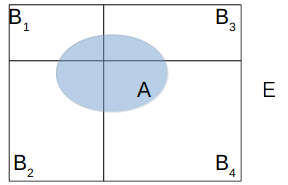
\includegraphics[width=0.51\columnwidth]{A.imagenes/ACV-BioSan-Estat-Bayes.png}
        \caption[Representación geométrica del teorema de Bayes]{Representación geométrica del teorema de Bayes.}
    \end{figure}
\end{multicols}
\section{Combinatoria}
La Combinatoria es la parte de las matemáticas que estudia las técnicas de recuento, en particular, las distintas formas de seleccionar subconjuntos de elementos de un conjunto según unos criterios.
\subsection{Números combinatorios}
El número combinatorio ${n \choose k}$ se define como el número de subconjuntos de $n$ tomados de $k$ en $k$, sin importar el orden y sin repetición. Se calcula como:
\begin{center}
    \begin{equation}
        {n \choose k} = \dfrac{n!}{k!\cdot \left( n - k\right)! }
    \end{equation}
    \captionof{Ecuacion}[Números combinatorios]{Números Combinatorios: Se distinguen cuatro casos especiales:\protect\\
        ${n \choose n} = 1; {n \choose 0} = 1; {n \choose 1} = n; {n \choose n-1} = n$.}
\end{center}
\subsection{Variaciones}
\subsubsection{Variaciones sin repetición}
Se obtiene el número de grupos distintos que se pueden formar con $n$ elementos de forma que cada grupo esté formado por $p$ elementos distintos y que dos grupos son distintos si algún elemento difiere en el orden o en el elemento en sí.
\begin{center}
    \begin{equation}
       V_{n,p} = n - \left( p + 1\right) 
    \end{equation}
    \captionof{Ecuacion}[Variaciones sin repetición]{Variaciones sin repetición.}
\end{center}
\subsubsection{Variaciones con repetición}
Se obtiene el número de grupos distintos que se pueden formar con $n$ elementos de forma que cada grupo esté formado por $p$ elementos repetidos o no y que dos grupos son distintos si algún elemento difiere en el orden o en el elemento en sí.
\begin{center}
    \begin{equation}
        VR_{n,p} = n^p
    \end{equation}
    \captionof{Ecuacion}[Variaciones con repetición]{Variaciones con repetición.}
\end{center}
\subsection{Permutaciones}
\subsubsection{Permutaciones sin repetición}
Se definen diferentes grupos de $n$ elementos distintos que se pueden formar si la diferencia radica en el orden de los mismos.
\begin{center}
    \begin{equation}
        P_n = n!
    \end{equation}
    \captionof{Ecuacion}[Permutaciones sin repetición]{Permutaciones sin repetición.}
\end{center}
\subsubsection{Permutaciones con repetición}
Se definen diferentes permutaciones de $n$ elementos en los que los diferntes elementos se repiten $a, b, \dots k$ veces, respectivamente
\begin{center}
    \begin{equation}
        P_n = \dfrac{n!}{a!\cdot b! \dots k!} \iff a + b +\dots + k = n
    \end{equation}
    \captionof{Ecuacion}[Permutaciones con repetición]{Permutaciones con repetición.}
\end{center}
\section{Variables aleatorias}
Una variable aleatoria ($X$) es una función o fórmula que le asigna a cada elemento $p$ del espacio muestral $\Omega$, un número real ($\R$), llamado ($X_p$). Son siempre cuantitativas, definiéndose como modelo teórico. La función de una variable aleatoria definen sucesos probabilisticos (subconjunto de elementos del espacio muestral) cuando se les asigna un valor, luego la imagen de $X_p$ es la probabilidad de $p$ en la variable $X$. Existen dos tipos:
\begin{itemize}[itemsep=0pt,parsep=0pt,topsep=0pt,partopsep=0pt]
    \item \textbf{Variable aleatoria discreta}: aquella que toma un número finito de valores.
    \begin{figure}[H]
        \centering
        \begin{equation*}
            \begin{split}
                f: \N &\longrightarrow \left[ 0, 1\right] \\
                x_i &\longrightarrow f\left( x_i\right) = P _{\left[ X = x_i\right]} = P _{\left[ e, t.q. X_{\left( e\right)}=x_i \right]}\\
            \end{split}
        \end{equation*}
    \end{figure}
    \item\textbf{Variable aleatoria continua}: aquella que puede tomar un infinito no numerable de valores.
    \begin{figure}[H]
        \centering
        \begin{equation*}
            \begin{split}
                f: \R &\longrightarrow \left[ 0, 1\right] \\
                x_i &\longrightarrow F\left( x\right) = P _{\left[ X \leq x \right]} = \int_{-\infty}^{\infty} f\left( t\right) \cdot dt
            \end{split}                
        \end{equation*}
        \caption*{Variable aleatoria discreta}
    \end{figure}
\end{itemize}
\subsection{Distribución Bernuilli y Binomial}
\subsubsection{Distribución de Bernuilli}
Sea una variable continua $X$, consiste en la realización de un experimento aleatorio con dos posibilidades, éxito o fracaso. La probabilidad de éxito es $p$ y la de fracaso es $q$, que se obtiene de $1-p$. 
\begin{table}[H]
    \begin{tabular}{cc}
        \rowcolor{black}\textcolor{white}{\textbf{Valor}}&\textcolor{white}{\textbf{Probabilidad}}\\
        1&$p$\\
        \rowcolor{hiperlightgray}0&$q = 1-p$\\
        \hline
    \end{tabular}
    \caption[Ejemplo de distribución de Bernuilli]{Ejemplo de distribución de Bernuilli $\left( X\rightarrow \mbox{Ber}_{\left( p\right)} \right)$. En este caso, 1 es \textit{Éxito} y 0 es \textit{Fracaso}. Un ejemplo es el lanzamiento de monedas, siendo 1 sacar cara y 0 no sacar cara.}
\end{table}
\subsubsection{Distribución binomial}
Sea una variable continua $X$ que es una suma de distribuciones de Bernuilli, es decir, consiste en la realización de experimentos aleatorios con varias posibilidade4s, cada una con su probabilidad correspondiente.
\begin{multicols}{2}
    \begin{table}[H]
        \begin{tabular}{cc}
            \cellcolor[HTML]{000000}{\color[HTML]{FFFFFF} Valor} & \cellcolor[HTML]{000000}{\color[HTML]{FFFFFF} Probabilidad}  \\
            $X_1$ & $P_{x_1}$   \\
            \rowcolor{hiperlightgray}$X_2$ & $P_{x_2}$   \\
            $X_3$ & $P_{x_3}$   \\
            \rowcolor{hiperlightgray}$\dots$ & $\dots$  \\
            $X_k$ & $P_{x_k}$ \\
            \hline
        \end{tabular}
        \caption[Ejemplo de distribución binomial]{Ejemplo de distribución binomial.}
    \end{table}
    \columnbreak
    \begin{center}
        \begin{equation}
            P_{\left( X\right) } = {n \choose k}\cdot P^k\cdot Q^{\left(  n-k\right) }
        \end{equation}
        \captionof{Ecuacion}[Formula de una ecuación binomial]{Formula de una ecuación binomial. De la fórmula de la izquierda se puede extraer: $P_{\left( X \right) }$: probabilidad de X; $n$: número total de elementos; $k$: número total de éxitos; $P$: Probabilidad de sacar el suceso; $Q$: Probabilidad de fracaso.}
    \end{center}
\end{multicols}
\subsection{Modelo teórico: media, varianza y dispersión}
Al ser modelos teóricos, existe la necesidad de contrastar estos datos con los reales, de forma que se verifique o no tal modelo.
\begin{itemize}[itemsep=0pt,parsep=0pt,topsep=0pt,partopsep=0pt]
    \item \textbf{Media teórica}: media más probable de obtener según una variable X.
    \begin{center}
        \begin{equation}
            \mu_X = \dfrac{\sum_{i}^{k}\left( P_{x_i}\cdot x_i\right) }{\sum_{i}^{k}P_{x_i}} \xrightarrow[]{\sum_{i}^{k}P_{x_i} = 1} \mu_X = \sum_{i}^{k} \left( P_{x_i}\cdot x_i\right) 
        \end{equation}
        \captionof{Ecuacion}[Formula de la media teórica]{Formula de la media teórica.}
    \end{center}
    \item \textbf{Varianza teórica}: varianza más probable de obtener según una variable X y su media teórica ($\mu_X$).
    \begin{center}
        \begin{equation}
            \sigma_X = \dfrac{\sum_{i}^{k}\left( P_{x_i}\cdot \left( x_i - \mu_X\right)^2\right)  }{\sum_{i}^{k}P_{x_i}} \xrightarrow[]{\sum_{i}^{k}P_{x_i} = 1} \sigma_X = \sum_{i}^{k} \left( P_{x_i}\cdot \left( x_i - \mu_X\right)^2\right) 
        \end{equation}
        \captionof{Ecuacion}[Formula de la varianza teórica]{Formula de la varianza teórica.}
    \end{center}
    \item\textbf{Coeficiente de variación teórico}: raíz cuadrada de la varianza teórica.
    \begin{center}
        \begin{equation}
            CV = \sqrt{\sigma_X} = \sqrt{\sum_{i}^{k} \left( P_{x_i}\cdot \left( x_i - \mu_X\right)^2\right) }
        \end{equation}
        \captionof{Ecuacion}[Formula del coeficiente de variación teórico]{Formula del coeficiente de variación teórico.}
    \end{center}
\end{itemize}
\begin{table}[H]
    \begin{tabular}{ccc}
        \rowcolor{black}&\textcolor{white}{\textbf{Variables de Bernuilli}}&\textcolor{white}{\textbf{Variables continuas}}\\
        Media teórica&$\mu_{\mbox{Ber}} = p$&$\mu_X = \int_{-\infty}^{\infty}x\cdot f\left( x\right) d\left( x\right) $\\
        \rowcolor{hiperlightgray}Varianza teórica&$\sigma_{\mbox{Ber}}^2 = p\cdot q$&$\sigma_X^2 = \int_{-\infty}^{\infty}\left( x -\mu_X\right) \cdot f\left( x\right) d\left( x\right) $\\
        Desviación teórica&$\sigma_{\mbox{Ber}} = \sqrt{p\cdot q}$&$\sigma_X =\sqrt{\int_{-\infty}^{\infty}\left( x -\mu_X\right) \cdot f\left( x\right) d\left( x\right)}$\\
        \hline
    \end{tabular}
    \caption[Definiciones teóricas de valores de centralización]{Definiciones teóricas de valores de centralización. Las variables de Bernuilli, al ser únicamente dos casos los posibles, las definiciones son sencillas; mientras que las variables continuas se definen mediante integrales.}
\end{table}
\subsection{Operaciones con variables aleatorias}
Toda variable aleatoria es en esencia una función cuya imagen asigna una probabilidad a un valor $x_i$. Al ser una función, también se le pueden sumar, restar, multiplicar y dividir números para obtener resultados proporcionales o hacer combinaciones lineales con otras funciones y obtener otra cualquiera.
\begin{equation*}
    X_{a,b}\xrightarrow{\exists}\left\lbrace \begin{array}{c}
        A\cdot X_{a,b}\\
        X_{a,b} + A\\
        X_{a,b}^A\\
        X_{1\left( a,b\right) } + X_{2\left( a,b\right) }\\
    \end{array}\right\rbrace 
\end{equation*}
Fuere cual fuere la operación practicada, la media, varianza y desviación típica de la función operada guardar una relación con la función no operada.
\begin{table}[H]
    \begin{tabular}{cccc}
        \rowcolor{black}&\textcolor{white}{$a,b$ números cualesquiera}&\textcolor{white}{$X_1,X_2$ variables dependientes}&\textcolor{white}{$X_1,X_2$ variables independientes}\\
        Media &$\mu_{a\cdot x+b} = a\cdot \mu_X + b$&$\mu_{X_1 + X_2} = \mu_{X_1} + \mu_{X_2}$&$\mu_{X_1 + X_2} = \mu_{X_1} + \mu_{X_2}$\\
        \rowcolor{hiperlightgray}Varianza &$\sigma_{a\cdot X + b} = a^2\cdot\sigma_X^2$&&$\sigma_{X_1 + X_2}^2 = \sigma_{X_1}^2 + \sigma_{X_2}^2$\\
        \hline
    \end{tabular}
    \caption[Operaciones con valores de centralización]{Operaciones con valores de centralización.}
\end{table}